\cotefile{64}
\scanpage{116}
% archive sheet number: 115
soit
\[
 \sigma_i z=\frac{\unsure{\zeta_i|\xi_i}z+\overbrace{\zeta_j\zeta_k-\zeta_i(\zeta_j+\zeta_k)}^{b_i}}{z-\zeta_i}
 \tag*{(61)}
\]
On peut transformer $b_i$, en utilisant les fonctions symétriques élémentaires $(-1)^\alpha a_\alpha$ des $\zeta$,
\[
 b_i=2\underbrace{\zeta_j\zeta_k}_{-a_3/\zeta_i}-
 (\underbrace{\zeta_i\zeta_j+\zeta_j\zeta_k+\zeta_k\zeta_i}_{a_2})
 =-(a_2+2a_3/\zeta_i)
\]
donc on trouve
\[
 \sigma_i z=\frac{\zeta_i z-(a_2+2a_3/\zeta_i)}{z-\zeta_i}
 =\frac{\zeta_i^2z-(a_2\zeta_i+2a_3)}{\zeta_i z-\zeta_i^2}
 \tag*{(62)}
\]
% slanted
\margin{expression valable du moins si $\zeta_i\ne0$, sinon on convient bien sûr que $a_3/\zeta_i$ \deleted{\unsure{se}} devient $\zeta_j\zeta_k$. Mais quitte à modifier en ajoutant une cte, \unsure{ts} les $\zeta_i\ne0$ \ldots}
Les \inserted{div. $\Delta_i$ des} points fixes de $\sigma_i$ est l'\deleted{ens} div. des solutions de l'équation en $z_i$
\[
 z_i^2-2\zeta_i z_i+(a_2+2a_3/\zeta_i)=0 \tag*{(63)}
\]
dont les solutions sont données par
\[
 z_i=\zeta_i\pm\sqrt{\underbrace{\zeta_i^2-a_2-2a_3/\zeta_i}_{\deleted{\unsure{\zeta}}}} \tag*{(64)}
\]
L'expression sous le signe $\sqrt{\vphantom{x}}$ s'écrit aussi
\[
 \frac{1}{\zeta_i}(\zeta_i^3-a_2\zeta_i-2a_3)
\]
ou encore, compte tenu de (66)
\[
 \zeta_i^3=-a_1\zeta_i^2-a_2\zeta_i-a_3
\]
\deleted{ce radical} cette expression devient
\[
 -\frac{1}{\zeta_i}(a_1\zeta_i^2+2a_2\zeta_i+3a_3)
\]
donc (\unsure{64|69}) s'écrit aussi
\[
 \left\{\begin{aligned}
 (z_i-\zeta_i)^2&=-\frac{1}{\zeta_i}(a_1\zeta_i^2+2a_2\zeta_i+3a_3)\\
 \text{i.e}\quad z_i&=\zeta_i\pm\sqrt{-\tfrac1{\zeta_i}(a_1\zeta_i^2+2a_2\zeta_i+3a_3)}
 \end{aligned}\right. \tag*{\textcircled{65}}
\]
% slanted
\margin{Si $\zeta_i=0$, on \deleted{\unsure{effectuera division}} \inserted{écrit} $-(a_1\zeta_i+2a_2+3\zeta_j\zeta_k)$ l'expr. sous le radical.}
Les douze \unsure{point|points} d'ordre $4$ de $E$ sont donc les points au dessus des six points $z_i$, donc \deleted{définis par} \inserted{un tel}
\scanpage{117}
% archive sheet number: 116
point est obtenu, pour un $i$ et un $z_i$ fixé, par le choix d'un $z'_i$ satisfaisant
\[
 {z'_i}^{\,2}=\underbrace{z_i^3+a_1z_i^2+a_2z_i+a_3}_{(z_i-\unsure{\zeta_i|\xi_i})(z_i-\zeta_j)(z_i-\zeta_k)}. \tag*{(66)}
\]
Choisir, pour tt $i\in\unsure{I|J}$, un $x_i\in E(k)$ tel que
\[
 2x_i=\varepsilon_i \tag*{(67)}
\]
revient donc à choisir, pour tt $i$, \deleted{\unsure{des|les}} la quantité
\[
 \wp(x_i)=z_i \tag*{(68 a)}
\]
soumise à (65) \inserted{(2 choix possibles)}, et ensuite, la quantité $z'_i$
\[
 \wp'(x_i)=z'_i) \tag*{(68 b)}
\]
soumise à (66) -- ce qui fait quatre choix possibles pour tt $i$, comme il se doit (car l'indétermination pour $x_i$ est dans $\vphantom{E}_2E(k)$).

Ceci posé, la condition d'épinglage de Jacobi relatif d'échelon $4$
\[
 \sum_{i\in I}x_i=0 \tag*{(69)}
\]
s'exprime par la condition
\[
 \left\{\begin{aligned}
 &\det\begin{pmatrix}1&z_1&z'_1\\1&z_2&z'_2\\1&z_3&z'_3\end{pmatrix}=0\qquad\text{i.e.}\\
 &(z_1z'_2-z_2z'_1)+(z_2z'_3-z_3z'_2)+(z_3z'_1-z_1z'_3)=0.
 \end{aligned}\right. \tag*{(70)}
\]
(cf prop. \unsure{33|3)}, qui s'applique, car les $x_i$ sont tous distincts. --)
\scanpage{118}
% archive sheet number: 117
En mettant ensemble les équations pertinentes : --
\margin{$z_i^2=2\unsure{\zeta_i|\xi_i}z_i-(a_2+2\zeta_j\zeta_k)\ \Longleftrightarrow$}
\[
 \left\{\begin{aligned}
 &(z_i-\zeta_i)^2=-\tfrac1{\zeta_i}(a_1\zeta_i^2+\unsure{2|L}a_2\zeta_i+3a_3)\quad [=-(a_1\zeta_i+2a_2+3\zeta_j\zeta_k)\\
 &{z'_i}^{\,2}=z_i^3+a_1z_i^2+a_2z_i+a_3\quad [=(z_i-\zeta_i)(z_i-\zeta_j)(z_i-\zeta_k)]\\
 &\det\begin{pmatrix}1&z_1&z'_1\\1&z_2&z'_2\\1&z_3&z'_3\end{pmatrix}=0\quad\text{i.e.}\quad
 \underbrace{(z_2z'_3-z_3z'_2)}_{\psi_1}+\underbrace{(z_3z'_1-z_1z'_3)}_{\psi_2}+\underbrace{(z_1z'_2-z_2z'_1)}_{\psi_3}=0
 \end{aligned}\right. \tag*{(71)}
\]
\margin{\uline{NB.} $[\psi_i^\omega=z_jz'_k-z_kz'_j\quad j=\omega i,\ k=\omega^2i=\omega j$}
qui expriment conjointement \deleted{\unsure{les|la}} donnée de $(x_i)_{i\in\unsure{I|J}}\in\unsure{\mathbb{E}|E}(k)^I$ satisfaisant (67) (69),
\[
 2x_i=\varepsilon_i\ (\in\phantom{E}_2E(k)^*),\qquad \sum x_i=0 \tag*{(72)}
\]
via
\[
 z_i=\wp(x_i),\quad z'_i=\wp'(x_i). \tag*{(73)}
\]

Je voudrais, à une telle donnée$_2$ $(x_i)_{i\in I}$, exprimée calculatoirement (via le choix d'un $\delta\in t_E^*$ et $\wp\in\unsure{\mathcal F_2|\mathscr F_2}$ associés) par (71), associer \inserted{canoniquement} un \uline{épinglage de Legendre de $E$}, de façon fonctorielle en $E$ et compatible avec les changem$^{\mathrm{ts}}$ de corps de base (entre autres\ldots). Je vais pour ceci supposer d'abord fixé un
\[
 \unsure{\mathbb{i}|\boldsymbol{i}|i|\dot{\imath}}\in\mu_4^*(k), \tag*{(74)}
\]
de sorte que, via ce choix, la première donnée $\alpha$ d'un épinglage de Legendre de $E$ s'interprète comme un élément
\[
 \omega\in\underline{\omega}=\underline{\omega}_I\qquad
 \begin{aligned}&\text{un ordre circulaire sur}\\ &I=\phantom{E}_2E(k)^*=\{\varepsilon_i\},\end{aligned}
 \tag*{(75)}
\]
% slanted
\margin{$\alpha=\mathbb{i}\wedge\omega$}
de sorte que la deuxième donnée $\kappa$ s'interprète comme un isomorphisme :
\[
 \kappa:\underline{t}_E\xrightarrow{\sim}\mathcal O_{\Sigma_I,t}(1)^{\unsure{\sharp|\natural}}
 \xrightarrow[\ ]{\inserted{\text{grâce au choix de }\mathbb{i}}\,\sim}\mathcal O_t(1),\tag*{(75)}
\]
\scanpage{119}
% archive sheet number: 118
satisfaisant à \unsure{la|\deleted{la}|\deleted{la}la} condition que son carré $\kappa^{\otimes2}$ s'\deleted{$\unsure{\kappa^{\otimes2}}$}identifie, via les isom. canoniques
\[
 \underline{t}_E^{\otimes2}\simeq T_{\Sigma_{\unsure{I|J}},t},\qquad
 \mathcal O_t(1)^{\otimes2}=\mathcal O_t(2)\underset{\text{via }\alpha}{\simeq}
 \mathcal O_t(2)(\underline\omega)\simeq T_{\Sigma_I,t} \tag*{(77)}
\]
à l'isom identique de $T_{\Sigma_I,t}$ -- ce qui, pour $\alpha$ fixé (deux choix), détermine $\kappa$ modulo signe. Pour $\alpha$ non fixé, $\kappa$ est déterminé modulo multiplication par $\mu_4(k)$.

Rappelons-nous de la suite exacte canonique
\diagram{\begin{tikzcd}[ampersand replacement=\&,column sep=small,row sep=small]
 (78) \& 0\arrow[r] \& F_t\arrow[r]\arrow[d,phantom,"\simeq"{description,rotate=90}] \& V_I(k)\arrow[r]\arrow[d,phantom,"\simeq"{description,rotate=90}] \& \mathcal O_t(1)\arrow[r] \& 0\\
 \& \& \mathcal O_t(-1)(\underline\omega) \& \Gamma(\Sigma_I,\underline{\mathcal O}_{\Sigma_I}(1))
\end{tikzcd}}
que \deleted{\unsure{par tenso}} je compare à
\diagram{\begin{tikzcd}[ampersand replacement=\&,column sep=small]
 (79) \& 0\arrow[r] \& k.1_{\Sigma_I}\arrow[r] \&
 \overbrace{\Gamma(\Sigma_I,\underbrace{\underline{\mathcal O}_{\Sigma_I}\{t\}}_{\substack{\simeq\underline{\mathcal O}_{\Sigma_I}(1)\\\text{non canoniquement}}})}^{\simeq\unsure{\mathcal F_2|F_2}}\arrow[r] \&
 T_{\Sigma_I,t}\arrow[r] \& 0
\end{tikzcd}}
On constate que la deuxième suite exacte est canoniquement isom. à celle déduite de la première, en la tensorisant par
\[
 \check F_t\simeq\mathcal O_t(1)(\underline\omega) \tag*{(\deleted{\unsure{79}}80)}
\]
(on a un iso valable chaque fois qu'on a un Module loc libre de rang $2$, $\underline V$, \deleted{\unsure{dont on|don}} \inserted{et} une section $t$ de $\mathbb P(\underline V)$ \ldots) :
\diagram{\begin{tikzcd}[ampersand replacement=\&,column sep=small,row sep=normal]
 \deleted{(\unsure{79|80})}(81) \& 0\arrow[r,dash] \& F_t\otimes\check F_t\arrow[r]\arrow[d,"\sim"] \& V_I(k)\otimes\check F_t\arrow[r]\arrow[d,"\sim"] \& \overbrace{\mathcal O_t(1)\otimes\check F_t}^{\underline{\mathcal O}_t(2)(\underline\omega)}\arrow[r]\arrow[d,"\sim"] \& 0\\
 \&0\arrow[r]\& k.1_{\Sigma_I}\arrow[r] \& \underbrace{\Gamma(\Sigma_I,\underline{\mathcal O}_{\Sigma_I}\{t\})}_{\unsure{\mathcal F_2}}\arrow[r]\&T_{\Sigma_I,t}\arrow[r]\&0.
\end{tikzcd}}
\scanpage{120}
% archive sheet number: 119
La donnée d'un isom $\kappa:\underline t_E\simeq\mathcal O_t(1)$ équivaut à celui de
\[
 \check\kappa:\underline{\check t}_E\simeq\underline{\mathcal O}_t(\unsure{+1|1})^\vee\simeq\underline{\mathcal O}_t(-1)
 \xrightarrow[\text{via }\omega]{}\underline{\mathcal O}_t(-1)(\underline\omega)\simeq F_t
\]
\deleted{ce qui implique une injection} \inserted{ou encore, à celui d'un} monomorphisme
\[
 \check t_E\hookrightarrow V_{\unsure{I|J}}(k)\hookrightarrow k^I
\]
dont l'image soit $F_t$, ou enfin à celui d'un élément non nul de
\[
 \deleted{\unsure{t_E}}\,V_I(t_E)=\deleted{\unsure{t_E^I}}\ \operatorname{Ker}(\underline t_E^I\xrightarrow[\text{somme}]{}\underline t_E)
\]
donc on peut considérer que la donnée de $\kappa$ revient à celle d'une famille
\[
 (\delta_i)_{i\in I}\in\underline t_E^I \tag*{(82)}
\]
satisfaisant certaines relations, savoir
\[
 \left\{\begin{aligned}
 &\text{a) }\sum\delta_i=0\quad\text{exprimant }\delta_i\in V_I(\underline t_E)\\
 &\text{b) Relation de proportionnalité, exprimant que}\\
 &\quad\text{l'image de }\check t_E\hookrightarrow V_I(k),\ \text{\unsure{défini|définie} par }(\delta_i)\text{ est }F_t,\\
 &\quad\text{de sorte que }(\delta_i)\text{ définit }\kappa:\underline t_E\simeq\check F_t\underset{\text{via }\omega}{\simeq}\mathcal O_t(1)\\
 &\text{c) Relation de l'épinglage de Legendre, exprimant}\\
 &\quad\text{que }\kappa^{\otimes2}\text{ est un isom. }\text{\unsure{standart|standard}}\text{ déjà connu.}
 \end{aligned}\right. \tag*{(83)}
\]
Nous allons expliciter les $\delta_i$ en termes du choix d'un $\delta\in\underline t_E^*$, \inserted{en plus \unsure{du|des} choix de $\omega\in\underline\omega$,} comme
\[
 \delta_i=\varphi_i^\omega(\delta)\delta\qquad\text{où}\qquad
 \begin{aligned}&\varphi_i^\omega(\delta)\in k^*\\ &(i\in I,\omega\in\underline\omega(I),\delta\in t_E^*)\end{aligned} \tag*{(84)}
\]
La condition d'invariance de $\delta_i$ p.r. au choix de $\delta$ s'exprime par la relation
\[
 \varphi_i^\omega(\lambda\delta)=\frac1\lambda\varphi_i^\omega(\delta) \tag*{(85)}
\]
\scanpage{121}
% archive sheet number: 120
la condition (83) a) s'exprime par
\[
 \sum_i\varphi_i^\omega(\delta)=0 \tag*{(86)}
\]
la condition b) par la condition
\[
 k.\big((\varphi_i^\omega(\delta))_i\big)=F_t \tag*{(87)}
\]
qui détermine d'emblée \deleted{les} $(\varphi_i^\omega(\delta))_i$ à scalaire inv. près -- la condition c les déterminant enfin (pour \uuline{$\unsure{\mathbb{i}|\boldsymbol{i}|i|\dot{\imath}}$} également choisi) au \uline{signe} près.

Bien sûr, \deleted{\unsure{on aura}} \inserted{la relation entre} $\kappa$ et les $\varphi_i^\omega(\delta)$ s'explicite par
\[
 (\varphi_i^\omega(\delta))=\underbrace{\check\kappa(\delta^{\unsure{\vee*|\vee}})}_{\mathcal O_t(-1)}\wedge\omega
 \ \in\mathcal O_t(-1)(\omega)\simeq F_t\subset V_{\unsure{I|J}}(k)\subset k^I \tag*{(88)}
\]
et la condition c) s'écrit Dieu sait comment -- il faudra \deleted{$\varphi_i^\omega(\delta)$} y revenir. Reste à exprimer la dépendance p.r. à $\omega$, pour \deleted{\unsure{exp|expr}} trouver l'invariance de l'épinglage de Legendre p.r. au choix de $\mathbb{i}$ i.e. p.r. au choix de $\omega=\omega_{\unsure{i|\mathbb{i}|\dot{\imath}}}$ ($\alpha:\mu_4^*(k)\simeq\underline\omega$ étant supposé déterminé), on trouve la relation nécessaire
\[
 \varphi_i^{\omega'}(\delta)=\deleted{\unsure{\mathbb{i}_\omega\alpha}}\mathbb{i}_\omega\varphi_i^\omega(\delta) \tag*{(89)}
\]
où
\[
 \mathbb{i}_\omega\overset{\text{déf}}=\alpha(\omega)\qquad
 \begin{aligned}
 &\alpha:\mu_4^*\simeq\underline\omega\text{ étant l'iso.}\\
 &\text{(supposé déterminé)}\\
 &\text{associé à l'épinglage}\\
 &\text{de Legendre cherché}
 \end{aligned}
\]
Posant
\scanpage{123}
% archive sheet number: 122
\diagram{\begin{tikzcd}[ampersand replacement=\&,column sep=small,row sep=small]
 \unsure{\zeta_1|\xi_1}\arrow[d,maps to]\&\zeta_2\arrow[d,maps to]\&\zeta_3\arrow[d,maps to]\&{}\in k\&\infty\arrow[dl,maps to,out=270,in=75]\\
 0\&1\&\infty\&t
\end{tikzcd}}
\[
 \left\{\begin{aligned}&\zeta_1,1\\&\zeta_2,1\\&\zeta_3,1\end{aligned}\right.
\]
\figure{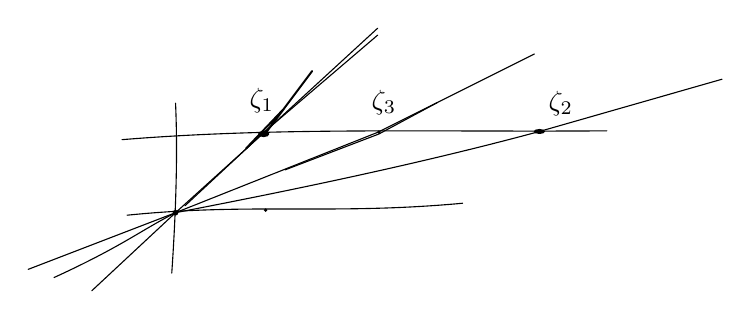
\begin{tikzpicture}[x=.008cm,y=.008cm,line cap=round,line join=round]
 \draw (-85,116) .. controls (160,136) and (398,128) .. (685,130);
 \draw (-77,-4) .. controls (120,16) and (250,-4) .. (456,15);
 \draw (-6,-96) .. controls (2,22) and (3,107) .. (0,174);
 \draw (-133,-124) -- (0,0) -- (137,124) -- (321,293);
 \draw[thin] (15,11) -- (143,130) -- (321,282);
 \draw[line width=.7pt] (112,102) -- (173,166) -- (142,125) -- (217,225);
 \draw (-193,-103) .. controls (-86,-54) and (-55,-28) .. (0,0) -- (322,128) -- (570,252);
 \draw[thin] (174,68) -- (323,125) -- (416,175);
 \draw (-234,-90) -- (0,0) .. controls (166,32) and (378,75) .. (578,129) -- (868,212);
 \fill (0,0) circle[radius=.036cm]; \fill (140,125) ellipse[x radius=.072cm,y radius=.040cm]; \fill (323,128) circle[radius=.024cm];
 \fill (578,129) ellipse[x radius=.072cm,y radius=.032cm]; \fill (143,4) circle[radius=.024cm];
 \node[above] at (137,143) {$\zeta_1$}; \node[above] at (331,140) {$\zeta_3$}; \node[above] at (612,138) {$\zeta_2$};
\end{tikzpicture}}
\[
 \begin{aligned}&\lambda_1\zeta_1,\lambda_1\\&\lambda_2\zeta_2,\lambda_2\\&\lambda_3\zeta_3,\lambda_3\end{aligned}
 \qquad\left[\begin{aligned}
 &\sum\lambda_i=0\\ &\sum\lambda_i\zeta_i=0\qquad \zeta_1,\zeta_2,\zeta_3\ \text{tous distinct}\\
 &\text{Cela détermine }(\lambda_i)\text{ mod }\inserted{\text{mult. par}}\text{ scalaire inv.}
 \end{aligned}\right.
\]
\[
 \begin{array}{rcl@{\qquad}|l}
 &&&\multicolumn{1}{l}{\unsure{01|O1}}\\
 \lambda_1&=&\zeta_{\underline2}-\zeta_{\underline3}&\zeta_1\\
 \lambda_2&=&\zeta_{\underline3}-\zeta_{\underline1}&\zeta_2\\
 \lambda_3&=&\zeta_{\underline1}-\zeta_{\underline2}&\zeta_3
 \end{array}
 \qquad\left\{\deleted{\Bigg\{}
 \begin{aligned}
 \unsure{e'_2|e_2}-e_3&=((\zeta_2-\zeta_3)\zeta_1,\zeta_2-\zeta_3)\\
 e_3-e_1&=((\zeta_3-\zeta_1)\zeta_2,\zeta_3-\zeta_1)\\
 e_1-e_2&=((\zeta_1-\zeta_2)\zeta_3,\zeta_1-\zeta_2)
 \end{aligned}\right.
\]
\[
 \deleted{\unsure{e_2}}\quad \deleted{f_1\longrightarrow}\qquad
 \deleted{(\zeta_1,1)\unsure{1|\mapstochar}\longrightarrow}\quad\zeta_1f_1+
\]
\scanpage{124}
% archive sheet number: 123
% letterhead
U N I V E R S I T E\\
DES SCIENCES ET TECHNIQUES\\
DU LANGUEDOC\\
\textasciicircum{}\textasciicircum{}\textasciicircum{}\textasciicircum{}\textasciicircum{}\textasciicircum{}\textasciicircum{}\textasciicircum{}\textasciicircum{}\textasciicircum{}\textasciicircum{}\textasciicircum{}

Montpellier, le 4 novembre 1980

\uline{Service de la Scolarité}

AM/gs

Diffusion : Liste A\\
N° 5791

\uline{AVIS DE SOUTENANCE D'UNE THESE DE DOCTEUR-INGENIEUR}

``\uline{SCIENCES DE L'EAU}''

% printed form
\uline{NOM et prénom du candidat} : PAPPALARDO Alain

\uline{Titre de la thèse} : ``Contribution à l'étude in situ des transferts de masse dans la zone non saturée des sols''

\uline{Date, heure et lieu de soutenance prévus} : Le 12 novembre 1980 à 10 heures

Salle de cours n° 9 - Université des Sciences et Techniques du Languedoc

\uline{Nom du Directeur de thèse} : M. C. BOCQUILLON

\uline{Désignation du Laboratoire où la thèse est préparée} : Laboratoire d'Hydrologie Mathématique. U.S.T.L. Montpellier.

\uline{Analyse de l'ouvrage} : Cette étude des phénomènes dispersifs lors d'un transfert de soluté dans un milieu poreux se décompose en trois parties:

a) Mise au point du principe d'utilisation d'une sonde prototype gamma/neutrons, susceptible de détecter la présence de deutérium dans l'eau du sol. Etalonnage et test de la méthode lors d'expériences de transferts d'eau deutérée sur la colonne de laboratoire.

b) Utilisation de cette méthode non destructice d'observation en continu de la solution du sol, pour obtenir des profils de concentration, lors de 5 expériences de transfert d'eau deutérée au champ, sur sol nu, en régime hydrodynamique permanent et transitoire et sur sol cultivé couvert de luzerne, sur le site expérimental de la ferme de Cadarache (C.E.A.).

c) Essais de modélisation des résultats expérimentaux obtenus in situ. Test de plusieurs modèles numériques du transfert d'eau et de soluté : modèle monodispersif et d'hétérogénéité. Utilisation de solutions analytiques plus simples à mettre en oeuvre.

\uline{Durée approximative des recherches ayant abouti à la thèse} : 3 ans

\uline{Composition du jury proposé} :

P/ le Secrétaire Général,\\
l'Attachée d'Administration\\
Universitaire,\\
\handwritten{\uline{\unsure{Gentil}}}\\
\uline{A. GENTIL}
\scanpage{125}
% archive sheet number: 124
\[
 \begin{aligned}
 \unsure{\zeta_1|\xi_1}f_1+f_2&=\frac1{\zeta_2-\zeta_3}(e_2-e_3)\\
 \zeta_2 f_1+f_2&=\frac1{\zeta_3-\zeta_1}(e_3-e_1)\\
 \zeta_3 f_1+f_2&=\frac1{\zeta_1-\zeta_2}(e_1-e_2)
 \end{aligned}
\]
\[
 \begin{aligned}
 (\zeta_1-\zeta_2)f_1&=\frac1{\zeta_3-\zeta_1}e_1+\frac1{\zeta_2-\zeta_3}e_2
 \deleted{\unsure{+}}\unsure{-|+}\left(\underbrace{\tfrac1{\zeta_3-\zeta_1}+\tfrac1{\zeta_2-\zeta_3}}_{\tikz[remember picture]\coordinate (carry125);}\right)e_3\\
 f_1&=\frac1{(\zeta_1-\zeta_2)(\zeta_3-\zeta_1)}e_1+\frac1{(\zeta_1-\zeta_2)(\zeta_2-\zeta_3)}e_2
 -\frac1{(\zeta_1-\zeta_2)}\big(\tikz[remember picture]\coordinate (into125);\phantom{xx}\big)e_3
 \end{aligned}
\]
\tikz[remember picture,overlay]\draw[->] (carry125) to[out=-15,in=75] (into125);
\[
 \begin{aligned}
 f_2&=\frac1{\zeta_2-\zeta_3}(e_2-e_3)-\zeta_1f_1\\
 &=-\frac{\zeta_1}{(\zeta_1-\zeta_2)(\zeta_3-\zeta_1)}e_1+
 \left(\frac1{\zeta_2-\zeta_3}-\frac{\zeta_1}{(\zeta_1-\zeta_2)(\zeta_2-\zeta_3)}\right)e_2\\
 &\qquad+\left[-\frac1{\zeta_2-\zeta_3}+\frac{\zeta_1}{\zeta_1-\zeta_2}
 \left(\frac1{\zeta_3-\zeta_1}+\frac1{\zeta_2-\zeta_3}\right)\right]e_3
 \end{aligned}
\]
\[
 \begin{aligned}
 (\zeta_1-\zeta_2)(\zeta_2-\zeta_3)(\zeta_3-\zeta_1)f_2
 &=-\zeta_1(\zeta_2-\zeta_3)e_1+
 \big[(\underset{\tikz[remember picture]\coordinate (dist125);}{\zeta_1}-\zeta_2)(\underset{\tikz[remember picture]\coordinate (toA125);}{\zeta_3}-\underset{\tikz[remember picture]\coordinate (toB125);}{\zeta_1})\\
 &\quad\deleted{\unsure{+}}\unsure{-|+}\zeta_1(\zeta_3-\zeta_1)\big]e_2+
 \big[\deleted{\unsure{+}}\unsure{-|+}(\zeta_1-\zeta_2)(\zeta_3-\zeta_1)\\
 &\quad+\zeta_1(\zeta_2-\zeta_3)+\zeta_1(\zeta_3-\zeta_1)\big]e_3
 \end{aligned}
\]
\tikz[remember picture,overlay]{\draw (dist125) to[bend right=22] (toA125);\draw (dist125) to[bend right=25] (toB125);}
\[
 -\zeta_1(\zeta_2-\zeta_3)e_1\unsure{-|+}\zeta_2(\zeta_3-\zeta_1)e_2-\zeta_3\rlap{\raisebox{1.5ex}{$\scriptscriptstyle/$}}(\zeta_1-\zeta_2)e_3\rlap{\raisebox{1.5ex}{$\scriptscriptstyle/$}}
\]
\scanpage{126}
% archive sheet number: 125
\[
 \deleted{\unsure{\zeta_1|\xi_1}(\zeta_2-\zeta_3)\qquad\zeta_2(\zeta_3-\zeta_1)}
\]
\[
 (\zeta_1-\zeta_2)(\zeta_2-\zeta_3)(\zeta_3-\zeta_1)=\unsure{\dot\Delta|\Delta}_0
\]
\[
 \boxed{\begin{aligned}
 -\Delta_0f_2&=\zeta_1(\zeta_2-\zeta_3)e_1+\zeta_2(\zeta_3-\zeta_1)e_2+\zeta_3(\zeta_1-\zeta_2)e_3\\
 \unsure{\cdot|-|{}}\,\Delta_0 f_1&=(\zeta_2-\zeta_{\unsure{3|2}})e_1+(\zeta_3-\zeta_1)e_2+(\zeta_1-\zeta_2)e_3
 \end{aligned}}
\]
$t$ correspond donc : $\sum(\zeta_j-\zeta_k)e_i$
\[
 =\sum_i(\wp(\varepsilon_j)-\wp(\varepsilon_k))e_i
\]
\scanpage{127}
% archive sheet number: 126
% letterhead
UNIVERSITE DES SCIENCES ET TECHNIQUES\\
DU LANGUEDOC\\
Institut de Mathématiques\\
Place Eugène Bataillon\\
34060 MONTPELLIER CEDEX

Dans le cadre des conférences d'intérêt général, Monsieur JAMBON parlera le Vendredi 12 décembre 1980, à 14h30, Salle de cours n° 4 sur le sujet suivant :

LES NOMBRES ENTIERS :

UNE PRESENTATION EN TERMES DE LANGAGE ALGORITHMIQUE

Vous êtes invité à cette conférence et au thé des mathématiciens qui suivra à 16 h dans la Salle de Réunion du Bâtiment de Mathématiques.

M. LEFRANC\\
Directeur de l'U.F.R. 5
\scanpage{128}
% archive sheet number: 127
Relations entre $M_{11}$ et $M_{04}$
\scanpage{129}
% archive sheet number: 128
(21 p)\qquad Approche transcendante
